\chapter{Software Requirements and System Design}

\section{Software Requirements}

The requirements should be defined correctly and briefly to design and implement a software product. In order to achieve this object, a detailed analysis is necessary. The following section will discuss the potential requirements from several different aspects.

\subsection{Main Function}
\label{req:main}

Initially, to figure out the requirements of a software product, the most vital work is ensuring this project's main function, or the primary target, and giving a brief description. Fortunately, the main function of this project is simple to summarise from the name, generating the signed distance field for arbitrary three-dimensional objects.

\hspace*{\fill}

Since the Wavefront OBJ has been chosen as the input file format in \ref{br:cmf}, the explanation can become more specific, generating SDF for triangular meshes. Therefore, the software is supposed to read in the data from .obj files and store the process of the information. Once the data has been stored in the memory, the software needs to analyse the data and compute signed distance functions, then store the result in a new file, and finally visualise the SDF on the screen.

\hspace*{\fill}

After defining the main requirement of this project, more specific demands need to be discussed. The following sections focus on more detailed aspects: Visualisation in \ref{req:visual}, GUI in \ref{req:gui}, Generation Algorithm in \ref{req:algo} and Evaluation in \ref{req:eva}.

\subsection{Visualisation}
\label{req:visual}

Before discussing the generation method requirement, as a computer graphic application, the contents of the graphic should be determined at first. The product should read in and visualise a triangle mesh as analysed in \ref{req:main}. Therefore, a camera and a simple scene are required to implement for rendering, which can be reused when rendering the SDF result. To visualise the SDF result, an intuitive solution is using different colours to represent the distance values; we can also use ray tracing or ray marching to test the practicality of SDF. The camera is supposed to observe the mesh from any angle, which can be implemented through a sphere orbit camera.

\subsection{Graphical User Interface}
\label{req:gui}

\begin{figure}[htbp]
    \centering
    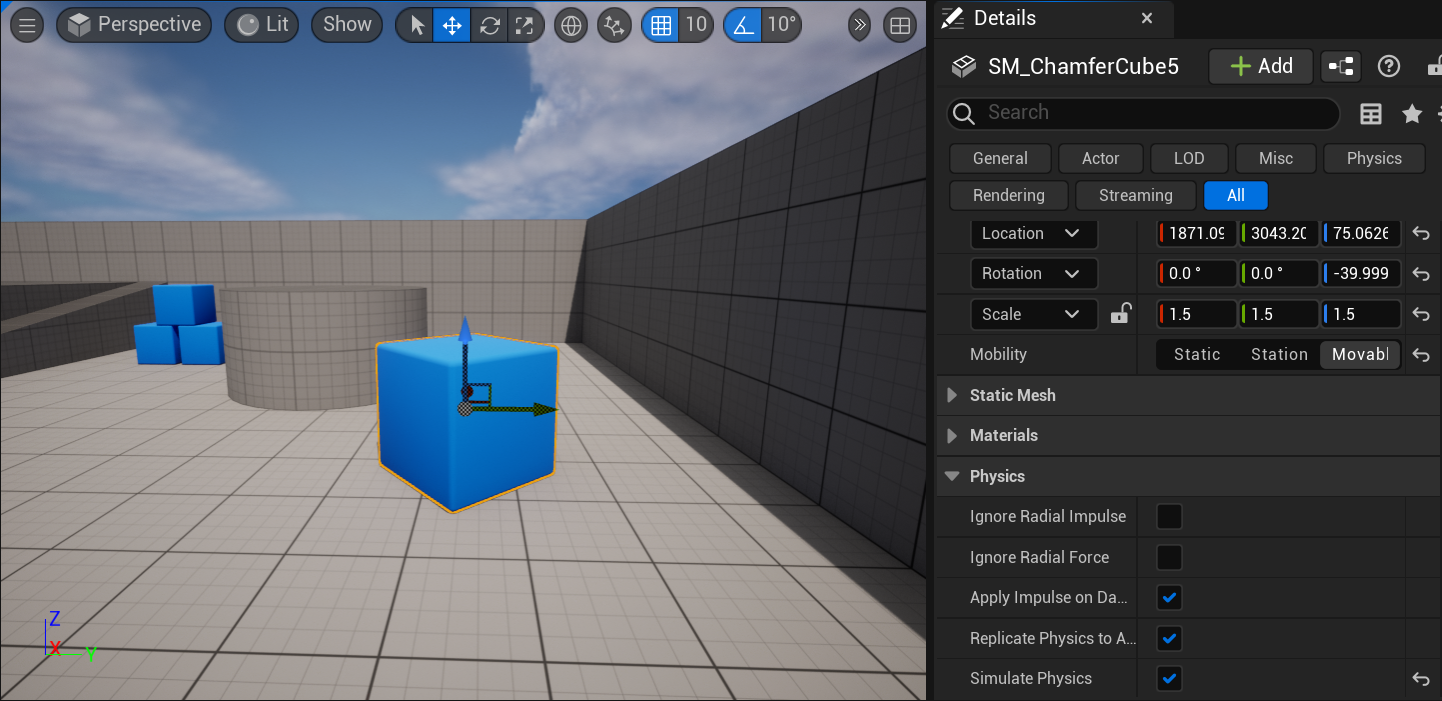
\includegraphics[width=16cm]{Images/Chap3/unreal.png}
    \caption{GUI screenshot of Unreal}
    \label{req:unreal}
\end{figure}

An appropriate graphical user interface is helpful for users to understand the functions the software product provides to them. Besides, the programmer can also complete the testing and debugging job through a well-designed GUI. Then we have to figure out what should a good interface looks like. The design of a successful commercial game engine inspires this question. As is shown in the screenshot of Unreal Engine (figure \ref{req:unreal}), the attributes of an object are illustrated on the GUI. In addition, the content of the visualisation can be changed through buttons and checkboxes. For this project, as discussed in \ref{req:visual}, the GUI is supposed to render a single model and its SDF in the same scene while the camera can move. Therefore, the requirement of an SDF generator GUI should contain the attributes info of the camera and several controls like checkboxes or buttons to change the visual contents of the object.

\subsection{Algorithm}
\label{req:algo}

The generation algorithm itself has been discussed in detail in the section \ref{br:algorithm1} and \ref{br:algorithm2} of Chapter \ref{chapter2}. The algorithm requirement should meet the choice mentioned in \ref{br:cAlgo}. Hence, two algorithms should be constructed for signed distance field computation, ray-tracing \cite{AkenineMller2005FastMS} and KD-tree. 

\subsection{Evaluation}
\label{req:eva}

As for evaluation, accuracy and efficiency should be considered. The result of the calculation should be saved as a text file to validate simply, while the efficiency can be evaluated through the time cost. 

\subsection{Others}

Other requirements like the multi-threading optimization should be applied to the computation process, and the project source code should be able to be compiled and running, as discussed in Chapter \ref{chapter2}. Those requirements will be considered in the system design.

\section{System Design}

\subsection{Overview}

According to the system requirement, this project will be divided into three main parts: GUI, algorithm and visualisation. In the GUI part, the Dear ImGui library will be used to implement a GUI class. In the algorithm part, three data structures of KD-Tree will be implemented as a class and used by the SDF calculation class. In the visualisation part, shaders, models, camera, and OpenGL render application is necessary for this project. Therefore, four classes will be implemented for each one. The software architecture of this project is shown in figure \ref{ds:archi}.

\begin{figure}[htbp]
    \centering
    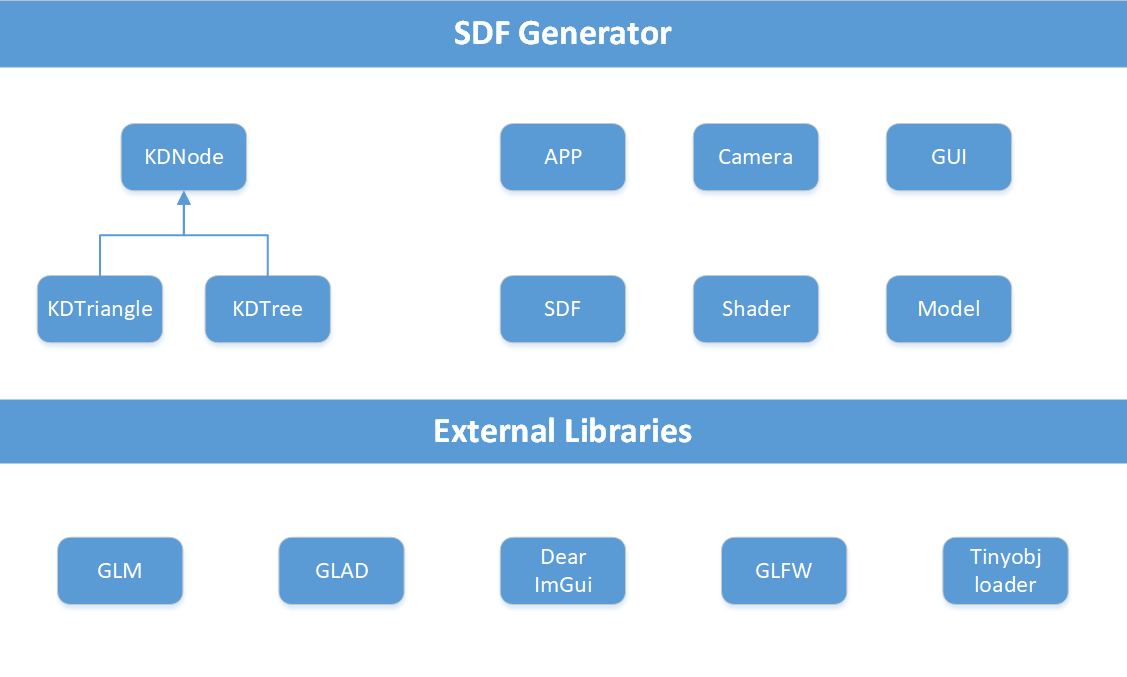
\includegraphics[width=16cm]{Images/Chap3/Architecture.png}
    \caption{The software architecture}
    \label{ds:archi}
\end{figure}

The detailed design of GUI, SDF algorithm and visualisation will be discussed in the following part of this chapter.

\subsection{Graphical User Interface}

As mentioned in \ref{br:ctpl}, the user interface will be implemented through Dear ImGui. ImGui is easily used to create a moveable control panel in front of the rendering widget. Therefore, the control options for rendering, the attributes of the camera and the debug info like generation time will be set on a moveable panel. The status of rendering control options can be changed through checkboxes. The GUI design is shown below in figure \ref{ds:gui}. 

\begin{figure}[htbp]
    \centering
    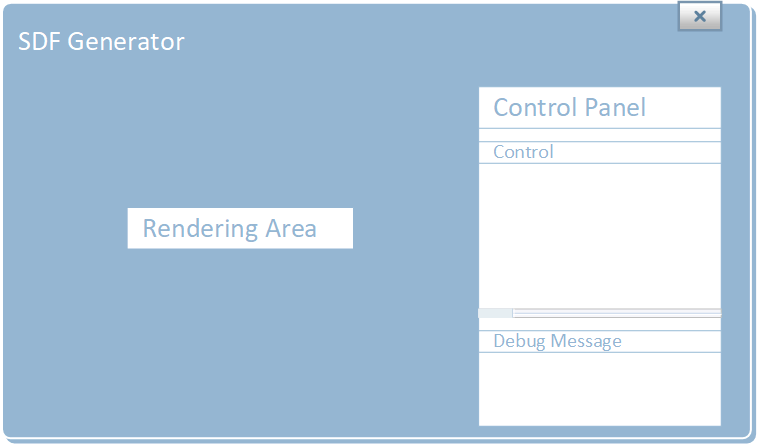
\includegraphics[width=15cm]{Images/Chap3/GUIdesign.png}
    \label{ds:gui}
    \caption{The application GUI design}
\end{figure}

\subsection{Algorithm}

There are three main algorithms to complete the signed distance field computation: the KD-tree structure, ray intersection and field generation.

\subsubsection{KD-Tree}
The tree should be built initially to use the KD-tree as the acceleration structure. As the project aims to generate a signed distance field for triangular meshes, the primitives of the tree should be triangles, which will be set as the tree node's data structure. Therefore, the nodes are constituted by the essential elements of triangles, i.e. vertices and edges. Besides, the bounding boxes and normal information will be stored in the nodes. To accelerate the process of ray intersection judgement, the function will be contained in the node structure.

\hspace*{\fill}

The structure of the KD-tree is shown in figure \ref{ds:kd}. The pseudocode of building the KD-tree algorithm is shown as Algorithm \ref{ds:kdbuild}.

\begin{figure}[htbp]
    \centering
    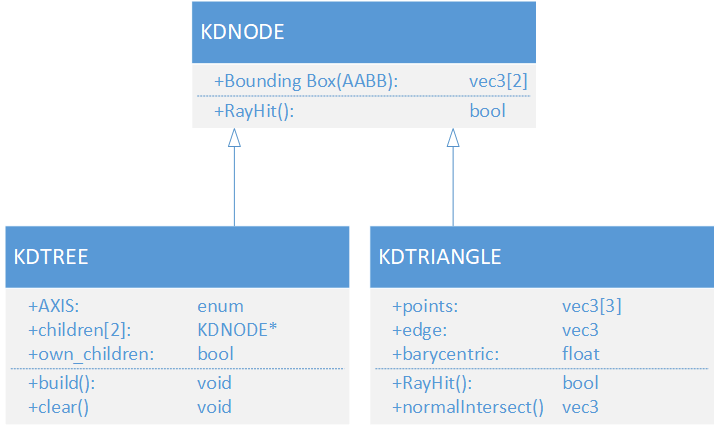
\includegraphics[width=15.5cm]{Images/Chap4/kdtree.png}
    \caption{The structure of KD-tree}
    \label{ds:kd}
\end{figure}

\subsubsection{Ray Instersection}

To apply the ray intersection algorithm, a number of sample rays must be generated equally. A sample voxel can be recognised as a sphere and split according to a fixed step. In Ahn's solution \cite{glsphere}, the sphere is divided into a number of stacks and sectors, shown as figure \ref{br:sphere}.

\begin{figure}[htbp]
    \centering
    \subfigure
    {
        \begin{minipage}[b]{.45\linewidth}
            \centering
            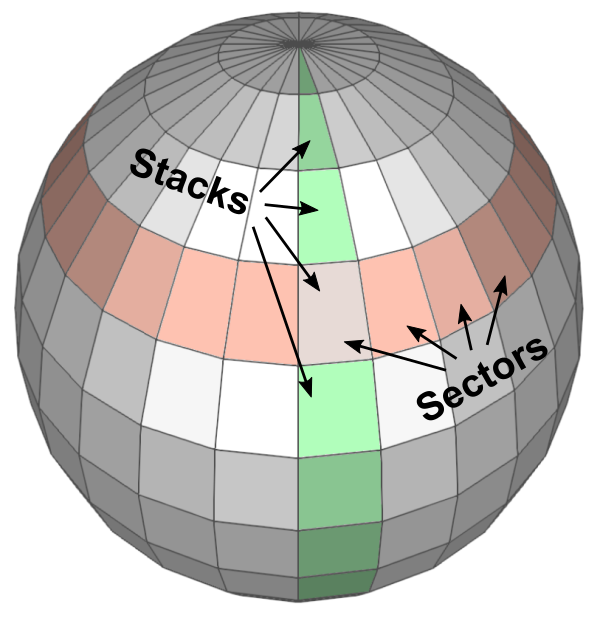
\includegraphics[width=6.5cm]{Images/Chap2/gl_sphere02.png}
        \end{minipage}
    }
    \subfigure
    {
         \begin{minipage}[b]{.45\linewidth}
            \centering
            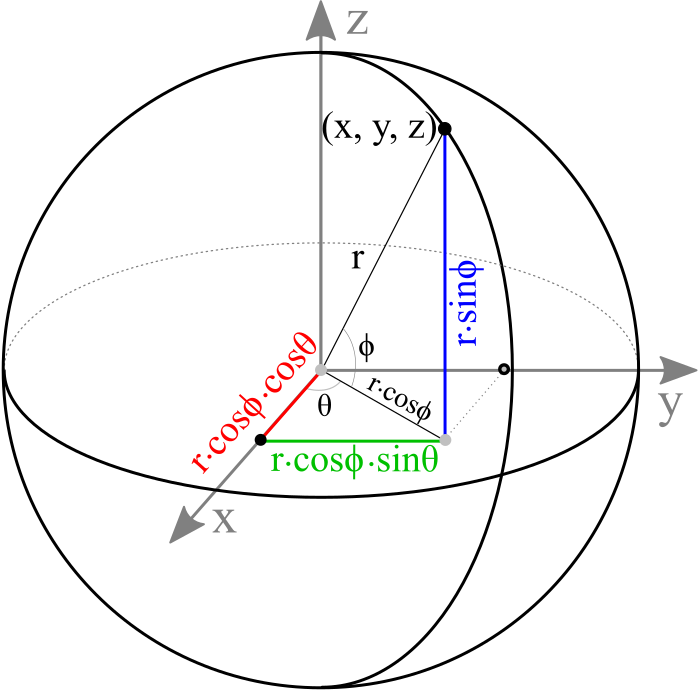
\includegraphics[width=6.5cm]{Images/Chap2/gl_sphere01.png}
        \end{minipage}
    }
    \caption{Calculate the coordinate of arbitrary point on sphere}
    \label{br:sphere}
\end{figure}

\clearpage

Then the coordinate of an arbitrary point p(x,y,z) can be computed as equation \ref{br:spherecoord}:

\begin{equation}
\label{br:spherecoord}
    \begin{aligned}
    x & = \left ( r\cdot \cos \phi  \right ) \cdot \cos \theta \\
    y & = \left ( r\cdot \cos \phi  \right ) \cdot \sin \theta \\
    z & = r\cdot \sin \phi 
    \end{aligned}
\end{equation}

Where the sector angle $ \theta $ and stack angle $ \phi $ can be calculated by equation \ref{br:sphereangle}:

\begin{equation}
\label{br:sphereangle}
   \begin{aligned}
    \theta & = 2\pi \cdot \frac{sectorStep}{sectorCount}  \\
    \phi & = \frac{\pi }{2} - \pi \cdot \frac{stackStep}{stackCount} 
    \end{aligned}
\end{equation}

\hspace*{\fill}

After generating the rays, the intersection algorithm needs to be used for distance computation. The algorithm of Tomas Akenine-M{\"o}ller and Ben Trumbore \cite{AkenineMller2005FastMS} represent a point on triangle as $ T(u, v)$, while $ (u, v) $ are the barycentric coordinates and satisfy $ u \geq 0, v \geq 0 $. Then $ T $ can be represent as \ref{br:pointT}:

\begin{equation}
    T(u, v)=(1-u-v) V_{0}+u V_{1}+v V_{2}
    \label{br:pointT}
\end{equation}

$ V_{0}, V_{1}$ and $ V_{2} $ are the vertices of triangle.

\hspace*{\fill}

We use $ R(t) $ to denote a ray of length t, then the formula for $ R(t) $ is as \ref{br:ray}:

\begin{equation}
    R(t)= O + t D
    \label{br:ray}
\end{equation}

$ O $ is the origin while $ D $ is the unit vector of direction.
Therefore, we can calculate the intersection problem by simply solving the equation \ref{br:intersection}:

\begin{equation}
    O+t D=(1-u-v) V_{0}+u V_{1}+v V_{2}
    \label{br:intersection}
\end{equation}

Which can be reordered as the linear system of equation\ref{br:interreoder}:
\begin{equation}
    \left[\begin{array}{lll}
        -D, & V_{1}-V_{0}, & V_{2}-V_{0}
        \end{array}\right]\left[\begin{array}{l}
        t \\
        u \\
        v
        \end{array}\right]=O-V_{0}
    \label{br:interreoder}
\end{equation}

let $ M=\left[-D, V_{1}-V_{0}, V_{2}-V_{0}\right] $, the ray and triangle can be transformed as \ref{br:trans}:
\begin{figure}[htbp]
    \centering
    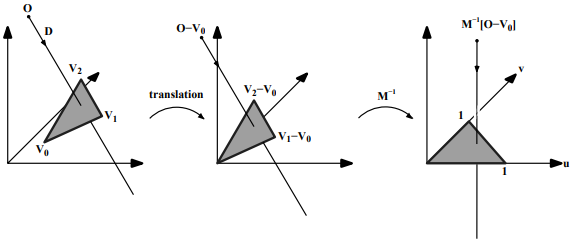
\includegraphics[width=15cm]{Images/Chap2/intersection.png}
    \caption{Translation and change of base of the ray origin}
    \label{br:trans}
\end{figure}

let $ E_{1}=V_{1}-V_{0}, E_{2}=V_{2}-V_{0} $ and $ T=O-V_{0} $, use the Cramer's rule, the equation \ref{br:interreoder} is able to be rearranged as \ref{br:reorder1}:

\begin{equation}
    \begin{bmatrix}t
        \\u
        \\v
       \end{bmatrix}=\frac{1}{\left|-D,E_{1},E_{2}\right|}
       \begin{bmatrix}\left|T,E_{1},E_{2}\right| 
        \\\left|-D,T,E_{2}\right|
        \\\left|-D,E_{1},T\right|
       \end{bmatrix}
    \label{br:reorder1}
\end{equation}

\hspace*{\fill}

Applying $ |A, B, C|=-(A \times C) \cdot B=-(C \times B) \cdot A $ to \ref{br:reorder1}, we finally get equation \ref{br:interFinal}:

\begin{equation}
    \begin{bmatrix}t
        \\u
        \\v
       \end{bmatrix}
       =\frac{1}{\left (D\times E_{2}\right)\cdot E_{1}}
       \begin{bmatrix}\left( T\times E_{1}\right)\cdot E_{2} 
        \\\left (  D\times E_{2}\right )\cdot T 
        \\\left (  T\times E_{1}\right )\cdot D
       \end{bmatrix}
       =\frac{1}{P\cdot E_{1}} \begin{bmatrix}Q\cdot E_{2} 
        \\P\cdot T 
        \\Q\cdot D
       \end{bmatrix}
    \label{br:interFinal}
\end{equation}

where $ P=\left(D \times E_{2}\right) $ and $ Q=\left(T \times E_{1}\right) $.

Finally, the distance t can be calculated as \ref{br:distance}:

\begin{equation}
    t=\frac{Q\cdot E_{2}}{P\cdot E_{1}}
    \label{br:distance}
\end{equation}

There are two branches of the ray-intersection problem. The first one is to determine whether a ray intersects with the bounding box; id Software provides a solution in DOOM3 \cite{raybound}. If the ray intersects with the bounding box, then the application will make a further determination, which is the second branch: intersect with the triangle. This algorithm will be used in the second branch to compute the distance function.

\subsubsection{Signed Distance Field Generation}

Finally, the whole distance field can be generated with the values of signed distance functions. The method of ray intersection judgement should be implemented through KD-tree acceleration and invoked by the generation algorithm.

\hspace*{\fill}

The data members of the SDF class should contain the file path, bounding box, resolutions, distance values, and sample voxels that should be stored into vectors. Besides, a generating function is necessary, and the computed values should be able to output and read in again.

\hspace*{\fill}

Figure \ref{ds:sdfclass} provide the structure of SDF class.

\begin{figure}[htbp]
    \centering
    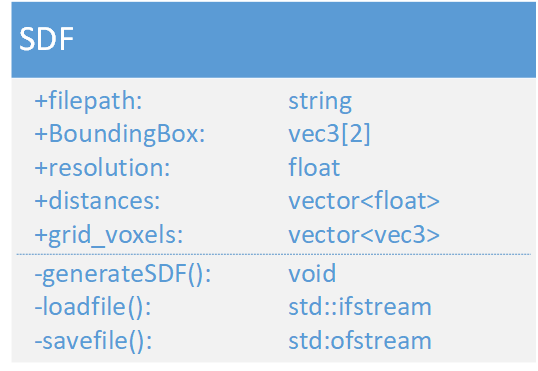
\includegraphics[width=10cm]{Images/Chap3/SDFclass.png}
    \caption{The structure of SDF class}
    \label{ds:sdfclass}
\end{figure}

\subsection{Visualisation}
\label{ds:visual}

The design of the visualisation module should contain resource loading (including shaders and models), a render scene, a scene camera and a render window.

\subsubsection{Resources Loading}
\label{ds:resource}

\paragraph{Shader}

The shader class should be about to load different types of shader files. Several enumerations can distinguish the shader type. After setting the type of shader, we can invoke the gl functions like glCompileShader() to compile shaders. Finally, the shader will be created successfully. 

\hspace*{\fill}

The structure of the shader class and its members are shown in figure \ref{ds:shaderclass}.

\begin{figure}[htbp]
    \centering
    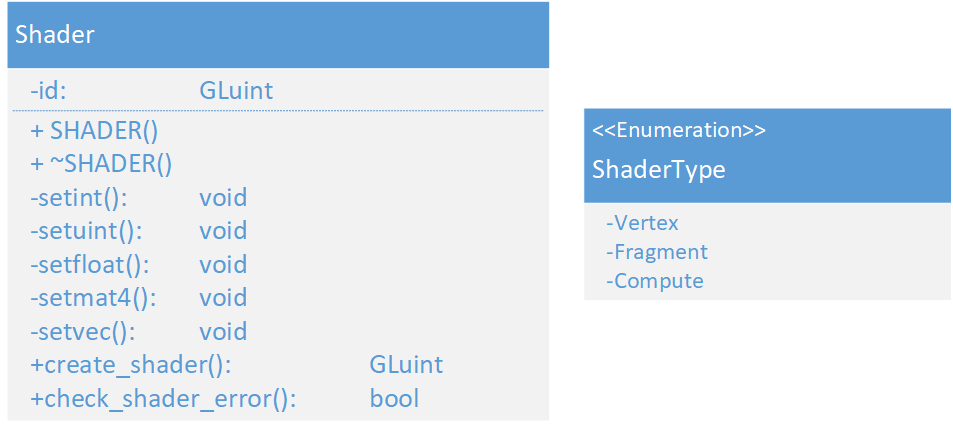
\includegraphics[width=16cm]{Images/Chap4/Shader.png}
    \caption{The structure of Shader class}
    \label{ds:shaderclass}
\end{figure}

\paragraph{Model}

The model load class used the tiniobjloader library. Considering about the requirements for computation, the information of vertices and normals will be read from the file. Then the vertices need to be reordered to the primitives, in this project, triangles. Then VAO and VBO should be created and allocated. Finally, the KD-tree should be built for the model, and the sample ray should test the intersection with the model. Therefore, both functions need to be implemented in the class.

\hspace*{\fill}

The structure of model class is shown in figure \ref{ds:modelclass}.

\begin{figure}[htbp]
    \centering
    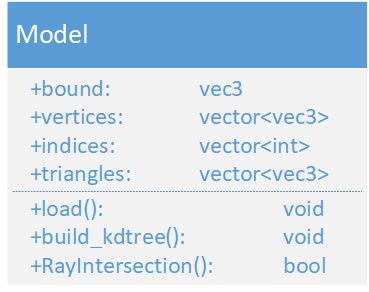
\includegraphics[width=8.5cm]{Images/Chap4/Model.png}
    \caption{The structure of Model class}
    \label{ds:modelclass}
\end{figure}

\subsubsection{Scene}

As for the scene, a grid-structured plane which can be extended infinitely is enough; the main coordinate axis will be highlighted. This plane can be implemented through a shader and can be directly reused by other applications or graphic APIs like Vulkan. Marie \cite{scene} provide the methods to create such a scene in the following order. First, create a basic grid plane vertex and fragment shader. Second, set the plane coordinates as infinity. Then draw the floor plane(i.e. y=0) and make the axis and grids on the floor. Finally, use the fragment shader to add a fade-out effect when the grid is far away.

\subsubsection{Camera}
\label{ds:camera}

The camera should be able to control by the mouse. The GLFW window will collect the user input; therefore, the camera class need to provide transformation functions like translation, rotation and zoom. Besides, the camera status should be updated by time step, and independent of the frame rate, the timer can be used for implementing the update method.

\clearpage

Figure \ref{ds:cameraclass} provides the structure of Camera class.

\begin{figure}[htbp]
    \centering
    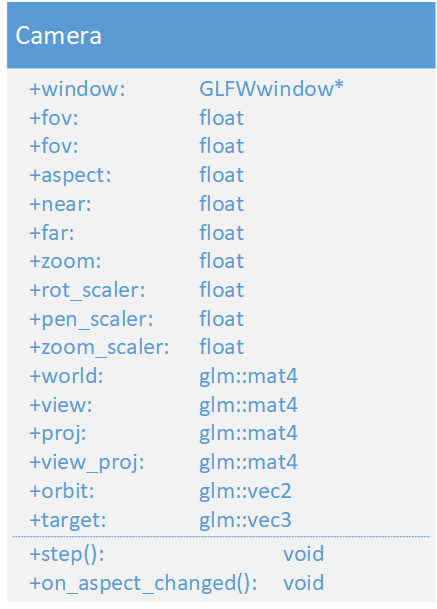
\includegraphics[width=10cm]{Images/Chap4/Camera.png}
    \caption{The structure of Camera class}
    \label{ds:cameraclass}
\end{figure}

\subsubsection{Rendering Process}
\label{ds:rendering}

The rendering process is divided into three main stages: initialize, terminate and rendering loop.

\paragraph{Initialize}

This stage contains the primary setting of an OpenGL application. A function for creating a GLFW window will be defined; other operations are contained in this function, like setting up a version and receiving the user input, which will be used to manipulate the camera. Besides, this function is also necessary for testing if the development environment has been set correctly. Then the rendering resources need to be read in, including models and shaders. If the last compute result of the signed distance field exists, it will also be loaded. If not, then the computation function will be running. Before entering the rendering loop, the parameters of the GUI will be set, and the GUI components will be bound to the same GLFW window.

\paragraph{Terminate}

The functions that tell the libraries to terminate and release the resources like glfwTerminate() have been contained in their codes, which only needs to be invoked by the terminate function.

\paragraph{Rendering}

In the rendering loop, three tasks need to be completed. First, the status of the timer needs to be stored and updated to ensure the camera transformation's stability. Then, the application will get framebuffer status and update continuously. For example, if the window has been resized, the viewport should be updated so that the pixels will be rendered properly; the swapbuffer technique \cite{Framebuffer} is applied in this process to prevent tearing or flickering issues. In addition, the GUI panel will be configured, and the contents like checkboxes and textboxes will be created and updated. Finally, the rendering function will bind different shaders when changing the modes of rendering.